\documentclass[11pt]{article}

\usepackage{fourier}
\usepackage{graphicx}
\graphicspath{{../../Figures/PDF/},{../../Figures/PNG/}}
\usepackage{natbib}
\usepackage{url}
\usepackage[a4paper]{geometry}

\title{Analysis of Handwritten Spirals}
\author{Alejandro C.\ Frery}
\date{DATA 301}

\begin{document}
\maketitle

\section{Introduction}

This project aims at starting an in-depth analysis of handwritten spirals, whose data were collected as part of a study with patients of Parkinson disease.

The initial scientific question is the following:
\begin{quote}
Which are good descriptors that allow discriminating from control and ill patients?
\end{quote}

In this first stage, the idea is to propose descriptors based on two examples, one control and one ill patient.

\section{Data}

Each patient is requested to draw a spiral between two guiding lines using a tablet.
The data consists of ASCII files with one header line containing the number of subsequent lines, followed by seven columns with the time-ordered
$x$ and $y$ coordinates,
the time stamp,
the on/off state of the pen,
the azimuth,
the altitude, 
and the pressure.
An example of the first ten lines of an actual file is the following:
\begin{verbatim}
4183
5310 3728 1845198 1 3280 810 238
5311 3726 1845206 1 3280 810 320
5311 3726 1845213 1 3280 810 302
5312 3725 1845221 1 3280 810 260
5313 3725 1845228 1 3280 810 244
5315 3724 1845236 1 3280 810 206
5317 3724 1845243 1 3250 810 216
5319 3724 1845251 1 3250 810 260
5319 3724 1845251 1 3250 810 260
\end{verbatim}

Fig.~\ref{Fig:AzimuthAltitude} illustrates what the azimuth and altitude of a pen measure.

\begin{figure}[hbt]
\centering
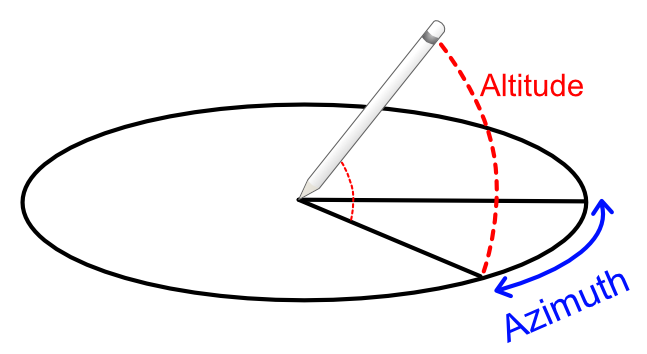
\includegraphics[width=.6\linewidth]{AzimuthAltitudeDiagram}
\caption{Azimuth and altitude of a pen (Source: \protect\url{https://www.raywenderlich.com/1407-apple-pencil-tutorial-getting-started}).}
\label{Fig:AzimuthAltitude}
\end{figure}

Fig.~\ref{Fig:ExampleSpirals} shows two examples of control spirals (produced by a healthy subject), and an example produced by an ill patient.

\begin{figure}
\centering
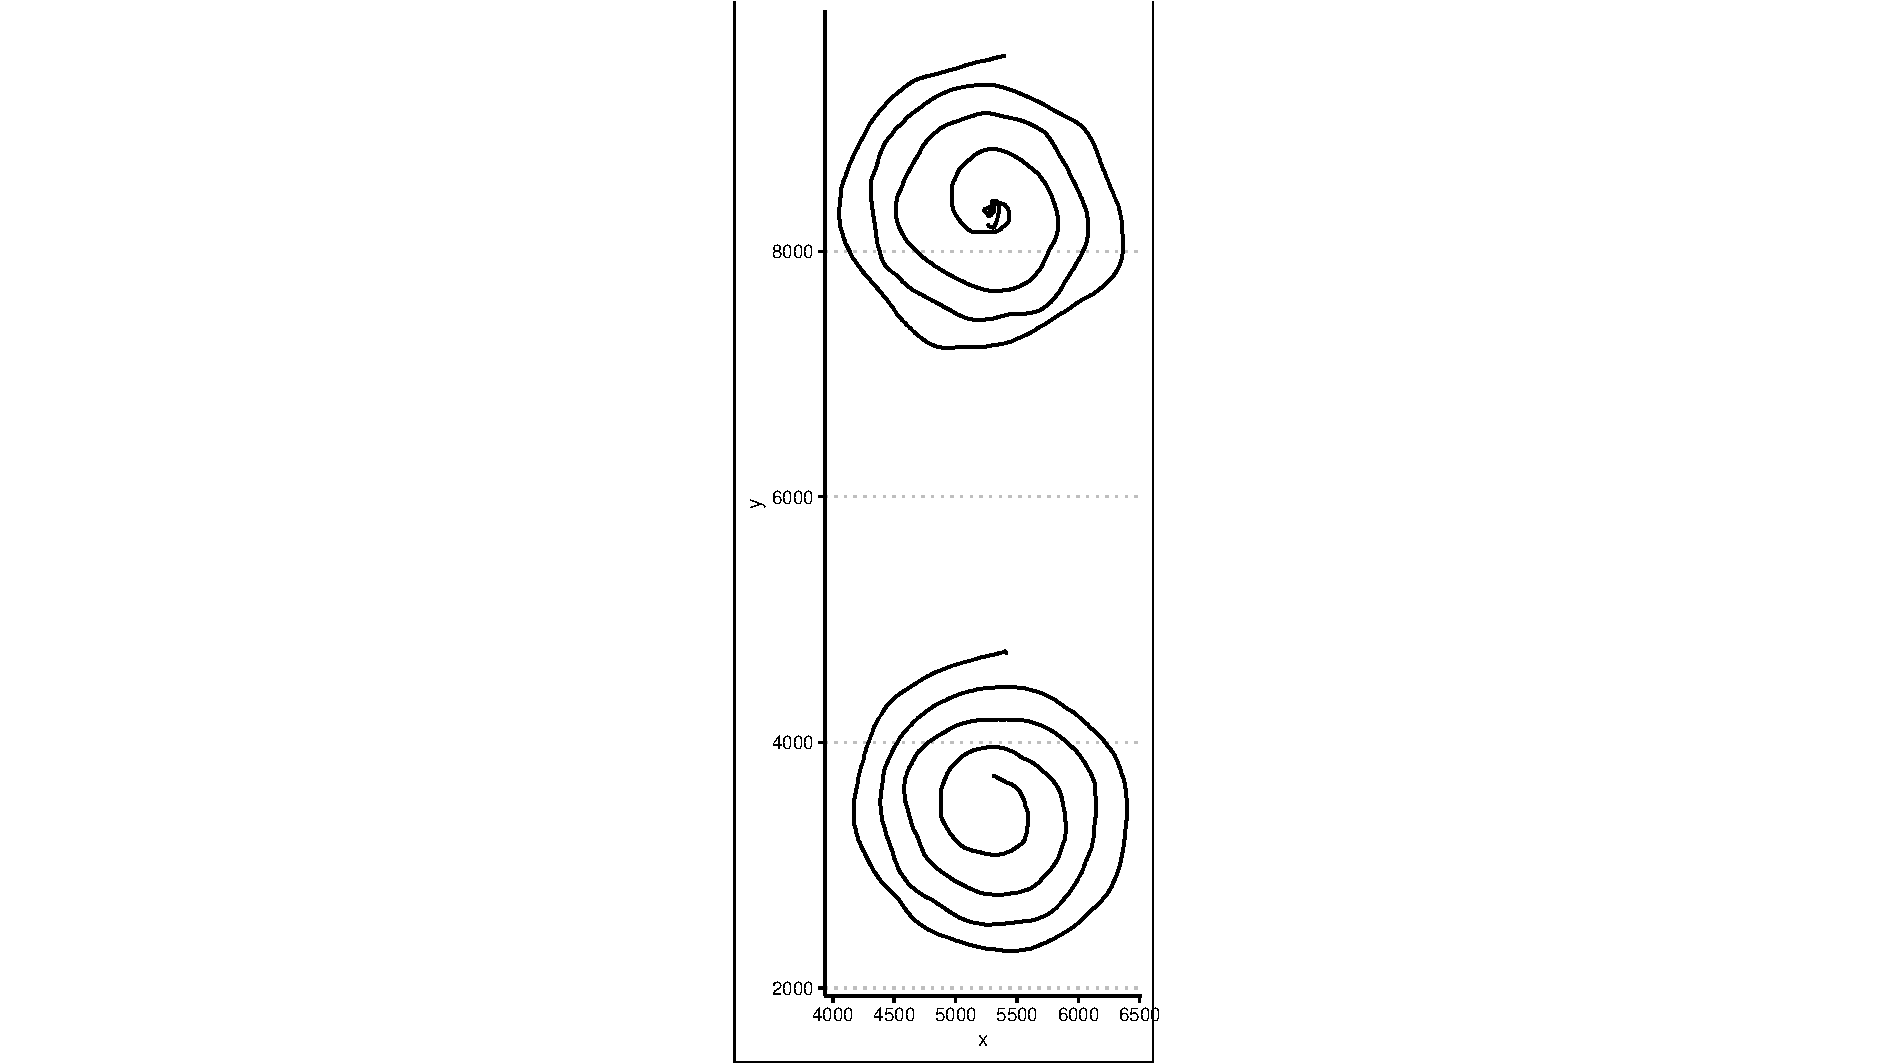
\includegraphics[width=.45\linewidth]{Control}
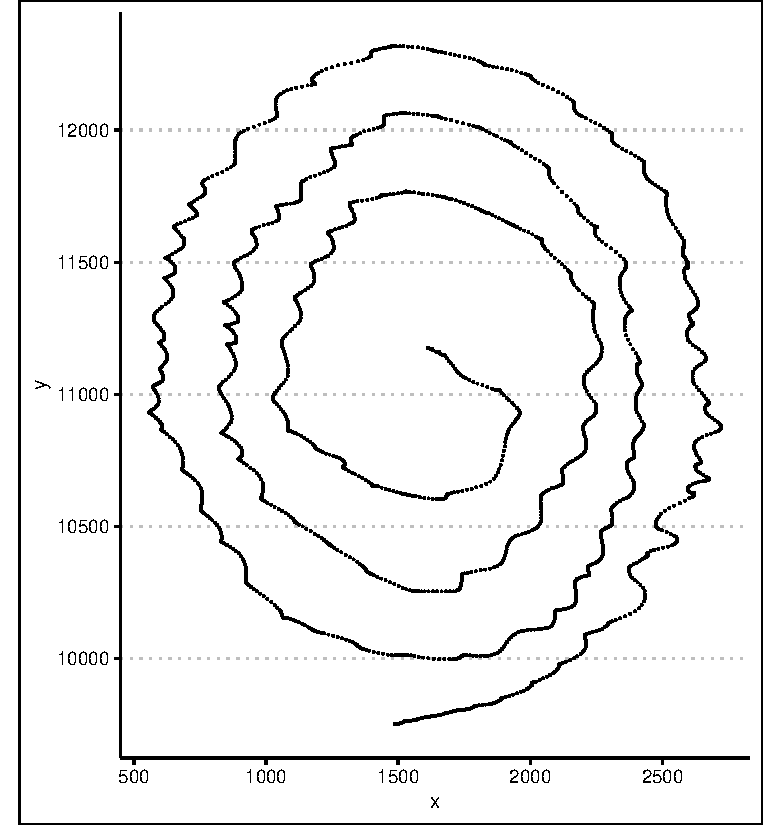
\includegraphics[width=.45\linewidth]{Ill}
\caption{Control (left) and ill (right) subjects results}\label{Fig:ExampleSpirals}
\end{figure}

These plots were produced with the following \texttt{R} code:

\begin{verbatim}
require(readr)
require(ggplot2)
require(ggthemes)

theme_set(theme_clean())

u00003s00002_hw00001 <- read_table2("u00003s00002_hw00001.svc", 
     col_names = FALSE, skip = 1)
names(u00003s00002_hw00001) <- c("x", "y", "Time", "On/Off", 
     "Azimuth", "Altitude", "Pressure")


ggplot(u00003s00002_hw00001, aes(x=x, y=y)) +
geom_point(size=.01) +
coord_fixed()

u00005s00001_hw00001 <- read_table2("u00005s00001_hw00001.svc", 
      col_names = FALSE, skip = 1)
names(u00005s00001_hw00001) <- c("x", "y", "Time", "On/Off", 
      "Azimuth", "Altitude", "Pressure")


ggplot(u00005s00001_hw00001, aes(x=x, y=y)) +
geom_point(size=.01) +
coord_fixed()
\end{verbatim}


\section{Starting point}

The reports should start by describing the source of the data, and concerns about patients' privacy.

As a mere suggestion, 
the project may start by rectifying the data by fitting it to a spiral data model~\citep[see, for instance,][]{AnAlgorithmforFittingArchimedeanSpiraltoEmpiricalData}, 
then by making an EDA, 
followed by classical time series analysis~\citep{IntroductoryTimeSerieswithR}, 
and by descriptors of statistical complexity~\citep{RepresentationSpaceTimeSeries}.


\bibliographystyle{kluwer}
\bibliography{books,articles}

\end{document}


